\documentclass[a4paper,12pt]{article}
\author{}

\usepackage[utf8]{inputenc}

\usepackage{amsmath}
\usepackage{amsfonts}
\usepackage{mathtools}
\usepackage{fixmath}
\usepackage{siunitx}

\usepackage{cancel}

\usepackage{graphicx}

\usepackage{subcaption}
\usepackage{caption}

\graphicspath{{figures/}}

\newcommand\norm[1]{\left\lVert#1\right\rVert}
\renewcommand{\vec}[1]{\boldsymbol{#1}}
\newcommand{\matr}[1]{\mathbf{#1}}
\newcommand{\unitvec}[1]{\hat{\mathbold{#1}}}
\newcommand{\unitvecg}[1]{\hat{\mathbold{#1}}}
\newcommand{\diff}{\mathop{}\!\mathrm{d}}
\newcommand{\cosine}[1]{\mathop{}\!\mathrm{c}_{#1}}
\newcommand{\sine}[1]{\mathop{}\!\mathrm{s}_{#1}}
\newcommand{\transpose}{^{\mathrm{T}}}
\newtheorem{principle}{Principle}
\newtheorem{prop}{Proposition}

\begin{document}

\tableofcontents
\newpage
\section{Background}
In this section some basics concepts related to the human walking are introduced. Later they will
be applied to the robot walking 
\subsection{Locomotion in human being}
The \emph{gait cycle} is defined as the time between two successive foot contact of the same limbs,
it can be divided in two phases, the \emph{Stance Phase}  and the \emph{Swing phase}.
For analyzing gait cycle one foot is taken as reference and its movements studied.
The Stance phase is the part of a gait cycle during which the foot remains in contact with the
ground, it constitutes about the $60\%$ of the gait cycle. In this phase five parts can be
distinguished:
\begin{itemize}
\item [-]\emph{Initial contact}: Instant the foot contacts the ground;
\item [-]\emph{Loading response}: Time period between the initial contact phase and the instant
  when the other foot lifts the ground;
\item [-]\emph{Mid stance}: Time interval from the end of the Loading response phase to the time
  when both ankles are aligned in the frontal plane;
\item[-]\emph{Terminal stance}: Period from ankles alignment to the contact of the swinging foot;
\item[-]\emph{Pre swing}: Time interval between the end of the terminal stance phase and the instant
  when the foot lifts from the ground.
\end{itemize}
The Swing phase is the phase of the gait during which the reference swings. It takes about $40\%$ of the gait cycle. Three parts can be distinguished:
\begin{itemize}
\item [-]\emph{Initial swing}: Phase during which the reference foot is lifted from the ground
  to position of maximum  knee flexion;
\item [-]\emph{Mid swing}: Time period between the initial contact phase and the instant when the other foot lifts the ground;
\item[-]\emph{Terminal swing}: Following vertical tibia position to just prior to initial contact.
\end{itemize}
Last but not least the concepts of Double and Single support are introduced. The first one refers to
the period during which boot feet are in contact with the ground while the other refers to interval when only one foot is in contact with the ground.
\par
In figure \ref{fig:gait-cycle} all the phases described above are shown. For each phase the type of support (single or double) is specified.
\begin{figure}[!ht]
  \centering
  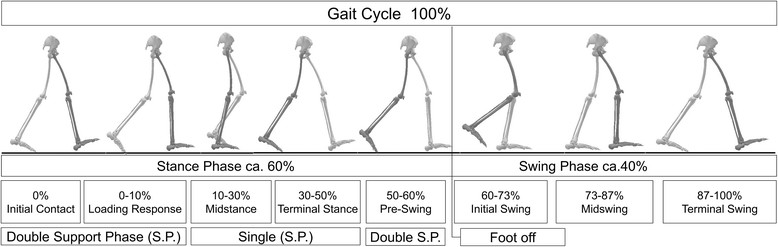
\includegraphics[scale=0.45]{gait-cycle.png}
  \caption{Classification of a human gait cycle. Image taken from \cite{Merker2015}. \label{fig:gait-cycle}}
\end{figure}
\par
In the following subsection the concepts described will be applied to the robot walking.
\subsection{Locomotion in robotic systems}
In robot locomotion the gait cycle described in the above section is simplified,
and the phases described are condensed in more general groups.
The walking task can be easy summarize using the \emph{walking cycle}
(Figure \ref{fig:walking_fsm}), it embeds all the phases of the human locomotion
shown in the figure \ref{fig:gait-cycle}. 
\begin{figure}[!ht]
  \centering
  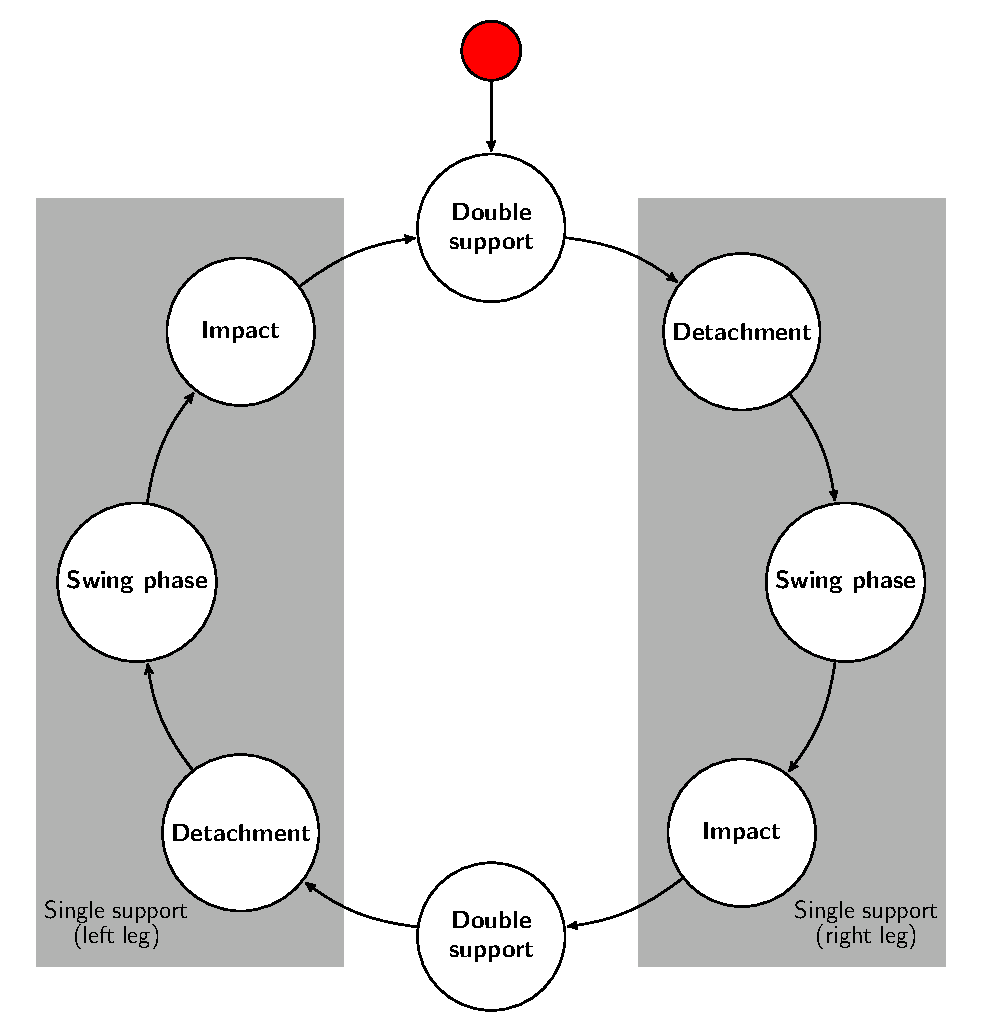
\includegraphics[scale=0.4]{walking_fsm}
  \caption{Walking cycle state machine. \label{fig:walking_fsm}}
\end{figure}
\par
The cycle can be split in two main phases, the Double support and the Single support ones.
The first one embeds the initial contact, the loading response and the pre swing phases while the
single support phase embeds the others.
During the SS phase the movement of the swing foot (i.e. the non reference foot)
is usually split in three sub-phases, \emph{detachment}, \emph{swing} and \emph{impact}.
More detailed:
\begin{itemize}
\item[-]\emph{Detachment}: Instant when the foot lifts from the ground;
\item[-]\emph{Swing}: this phase embeds the Initial swing, the mid swing and the terminal swing
  stages of the human walking;
\item[-]\emph{Impact}: Instant the foot contacts the ground.
\end{itemize}
In the following of this report only the single support phase is analyzed. Initially from the point
of view of the reference foot and the robot center of mass. Later the movement of the swing foot is
studied. 

\subsection{Zero Momentum Point}
In order to derive a model for the robot locomotion the \emph{zero momentum point} concept
\cite{Vukobratovic1969} must be discussed.
In the following dissertation only the single support phase is considered and in order to simplify the analysis only the support foot is considered.
\par
In the free body diagram of the reference foot (Fig \ref{fig:zmp_foot}) the influence of the
entire robot on the foot is replaced by the force applied to the point $A$
($\vec{F}_A$) and the torque relative to $A$ ($\vec{M}_A$) while the
total ground reaction consist on a force applied to the point $P$ ($\vec{R}$) and a torque
relative to $A$ ($\vec{M}$), finally the weight of the foot itself acts at its gravity center $G$.
\begin{figure}[!ht]
  \centering
  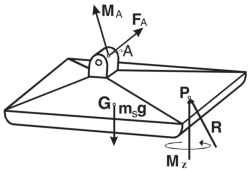
\includegraphics[scale=1.5]{zmp_foot}
  \caption{Free body diagram of the reference foot. Image edit from \cite{Vukobratov2004}. \label{fig:zmp_foot}}
\end{figure}
The horizontal components of the reaction force $\vec{R}$ ($R_x$ and $R_y$) are 
the friction force necessary to balance the horizontal components of the force $\vec{F}_A$, while
the vertical component of the reaction torque $\vec{M}$ ($M_z$) represents moment generated by the
friction reaction forces and it balances the vertical component of the torque $\vec{M}_A$.
In the following the reference foot is assumed in contact with the ground without sliding, therefore
the friction compensates the horizontal force components ($R_x$, $R_y$) and vertical reaction torque
($M_z$). The vertical reaction force $R_z$ compensates the vertical component of the force
$\vec{F}_A$ and the weight of the foot itself.  
\par
Finally it is very interesting to study the balancing of the horizontal component of the
torque $\vec{M_A}$ ($M_{A_x}$ and $M_{A_y}$). Because of the unilateral nature of the constraint between
the reference foot and the ground, these components can be only compensate by changing
the position of the point $P$ within the convex hull of the support polygon.
\par
In the Figure \ref{fig:zmp_foot_y} a simple planar case in sagittal plane is presented. In this
simple scenario the component $M_{A_x}$ is balanced by shifting the point $P$ 
\begin{figure}[!ht]
  \centering
  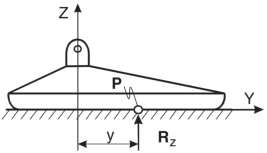
\includegraphics[scale=1.5]{zmp_foot_y}
  \caption{Example of a planar case. Image taken from \cite{Vukobratov2004}. \label{fig:zmp_foot_y}}
\end{figure}

It is important to note that all the time the reaction force $\vec{R}$ is within the support polygon
the ankle moment is full compensate by changing the position of the point $P$ and the horizontal
components of the interaction torque with the ground are zero. In the light of this statement in the
Figure \ref{fig:zmp_foot} only the component $M_z$ exists.
However, in the case which the sole is not large enough to allow the appropriate position of the
point $P$ the force $\vec{R}$ acts at the edge of the foot and the horizontal components $M_x$ and
$M_y$ are different from zero.
\par
The reasoning presented above can be summarized in the following principle \cite{Vukobratov2004}.
\begin{principle}
  The necessary and sufficient condition for the locomotion mechanism to be stable
  is that for the point $P$ on the sole where the ground reaction force is acting
  \[
  M_x = 0 \quad M_y = 0
  \]
\end{principle}
\subsubsection{Zero Momentum Point evaluation}
In this section the position of the zero momentum point is evaluated. It should be noted that the
prerequisite of the stability of the entire robot is the stability of the contact between the
reference foot and the ground. Thus for the supporting foot the following equations hold 
\[
\vec{R} + \vec{F}_A + m_s \vec{g} = \vec{0}
\]
\begin{equation}
  \label{eq:zmp_2_cardinal}
  \vec{OP} \times \vec{R} + m_s \vec{OG} \times \vec{g} + \vec{OA} \times \vec{F}_A + \vec{M}_A +
  \begin{bmatrix}
    0 \\
    0 \\
    M_z
  \end{bmatrix} = \vec{0}
\end{equation}
where $\vec{R}$, $M_z$, $\vec{F}_A$, $\vec{M}_A$ and $m_s$ are presented in Figure
\ref{fig:zmp_foot}, while $\vec{OP}$, $\vec{OG}$ and $\vec{OA}$ are respectively the position vector
from the origin of the coordinate system $O_{xyz}$ to the ground reaction force acting point ($P$),
CoM of the foot ($G$) and the ankle joint ($A$).
\par

Projecting the second cardinal equation (\ref{eq:zmp_2_cardinal}) onto the $z$-axis and placing the
origin of the reference system $O$ at $P$ (i.e. $O \equiv P$), $M_z$ can be evaluated
\[
M_z = M_{fr} = [-(\vec{M}_A + \vec{PA} + \vec{F}_A)]_z
\]
where $[\vec{v}]_z$ means $\langle \vec{v},\vec{e}_3 \rangle$.
\par
The projection of the equation (\ref{eq:zmp_2_cardinal}) onto the horizontal plane ($xy$-plane) gives
\[
\left[\vec{OP} \times \vec{R} + m_s \vec{OG} \times \vec{g} + \vec{OA} \times \vec{F}_A + \vec{M}_A\right]_{(x,y)} = \vec{0}
\]
placing the origin of the reference system $O$ at $P$ (i.e. $O \equiv P$) the following relation is
obtained
\begin{equation}
  \label{eq:zmp_eq}
  \left[ m_s \vec{PG} \times \vec{g} + \vec{PA} \times \vec{F}_A + \vec{M}_A\right]_{(x,y)} = \vec{0}
\end{equation}
An intuitive understanding is ob obtained by setting $m_s = 0$ and $\vec{M}_A = \vec{0}$ in equation
(\ref{eq:zmp_eq})
\[
\left[\vec{PA} \times \vec{F}_A\right]_{(x,y)} = \vec{0}
\]
in this particular case $P$ is the point on the ground where the line of the action of $\vec{F}_A$
penetrates (Figure \ref{fig:zmp_foot_y_example}).
\begin{figure}[!ht]
  \centering
  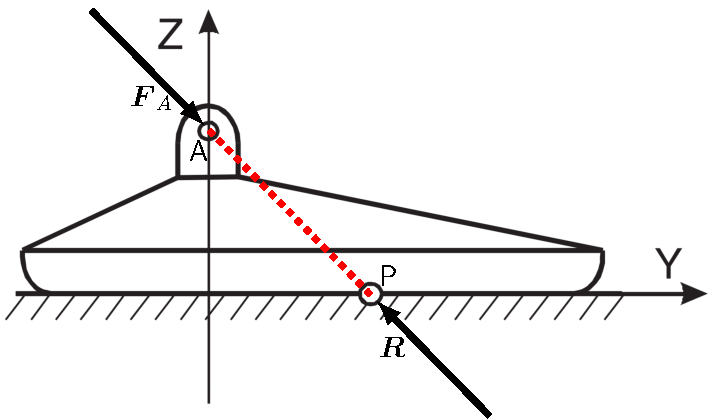
\includegraphics[scale=0.56]{zmp_foot_y_example}
  \caption{ZMP simple example. Image edit from \cite{Vukobratov2004}. \label{fig:zmp_foot_y_example}}
\end{figure}
The equation (\ref{eq:zmp_eq}) allows to evaluate the ZMP position. In order to understand if the robot
is in dynamic equilibrium the position of $P$ must be within the support polygon. However, in reality, the
point $P$ cannot exist outside the support polygon.
\par
The following principle holds:
\begin{principle}
  The position of the point $P$ is inside the convex hull of the support polygon ($\Omega$)
  IFF the robot is in dynamic equilibrium.
  \[
  P \in \Omega \longleftrightarrow \text{dyanamic equilibrium}
  \]
  \par
  However if the point $P \in \partial \Omega$ it is not possible to conclude on the stability of the robotic system.
  \par
  Where $\partial \Omega$ is the boundary of $\Omega$ (i.e. $\bar{\Omega} = \Omega \cup \partial \Omega$).
\end{principle}
Thus, in same case, the position of zero momentum point may not be enough to distinguish between a
stable walk and an unstable one, to solve this problem a new conpcet mus be introduced, the
Fictitious Zero momentum point, also know with the name of Foot Rotation Indicator (FRI)
\cite{Goswami1999}.
\newpage

\section{Derivation of the 3D-LIPM}
The motion of CoM and the reference foot can be modelled using two different approach.
In the first one the precise knowledge of robot dynamics
(mass of each joint, location of center of mass of each joint, etc.) is required.
The second approach, called \emph{inverted pendulum approach},
uses only a limited knowledge of the robot dynamics (the position of whole body center of mass
($CoM$), the entire mass of the robot ($m$), etc.). This last approach will be used in the following
report.
\par
The section is organized in two subsection, in the first one the equations of general 3D inverted
pendulum are shown. While in the other one the equations obtained are applied in the walking task.
\par
The following dissertation will be mainly based on Kajita's work \cite{Kajita2001}.
\subsection{Derivation of the equations of a general 3D Inverted Pendulum}
When a biped robot is supporting its body on one leg (i.e. the robot is
in the Swing phase), its dynamics can be approximated by the 3D Inverted Pendulum Model. This
approximation allows to reduce the dynamics of the whole body to a simple inverted pendulum
considering only the position of whole body center of mass ($CoM$) and
the entire mass of the robot ($m$).
\par
The model, shown in Figure \ref{fig:3d_lipm}, represents the entire robot as point mass in
top of a telescopic leg with no inertia while the other edge of this pendulum is the
``foot'', and it is set in rigid contact with the ground.
\begin{figure}[!ht]
  \centering
  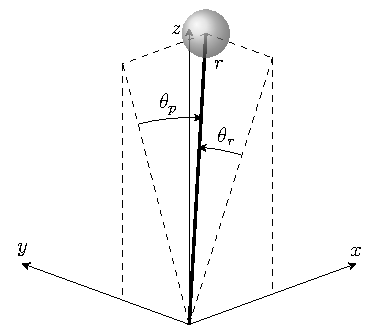
\includegraphics[scale=1.2]{3d_lipm}
  \caption{3D Inverted pendulum model. \label{fig:3d_lipm}}
\end{figure}
\par
The position of the mass point $\vec{p} = \begin{bmatrix} x & y & z \end{bmatrix} \transpose$
is uniquely specified by a set of the Lagrangian coordinates $\vec{q}$
\[
\vec{q} =
\begin{bmatrix}
  \theta_r & \theta_p & r
\end{bmatrix}\transpose
\]
where $r$ is the length of the pendulum while
the angles $\theta_r$ and $\theta_p$ are shown in the Figure \ref{fig:3d_lipm}.
\[
\begin{cases}
  x = r \sine{\theta_p}\\
  y = -r \sine{\theta_r}\\
  z = r \sqrt{1-\sine{\theta_r}^2-\sine{\theta_p}^2}
\end{cases}
\]
In order to develop a model of the pendulum the dynamic equation can be be easily derived
\begin{equation}
  \label{eq:3d_ip_inverseJ}
  m \ddot{\vec{p}} = (J\transpose)^{-1} \vec{\tau}  + m \vec{g}
\end{equation}
where $\vec{g} = \begin{bmatrix} 0 & 0 & -g \end{bmatrix} \transpose$ is the gravity vector,
$\vec{\tau} = \begin{bmatrix} \tau_r & \tau_p & f \end{bmatrix} \transpose$ is the actuated
force/torque vector associated to the Lagrangian coordinates and $J$ is the Jacobian matrix
\[
J = \frac{\partial \vec{p}}{\partial \vec{q}} =
\begin{bmatrix}
  0 & r \cosine{\theta_p} & \sine{\theta_p}\\
  -r\cosine{\theta_r} & 0 & - \sine{\theta_r}\\
  -\frac{r \cosine{\theta_r} \sine{\theta_r}}{\sqrt{1-\sine{\theta_r}^2-\sine{\theta_p}^2}} &   -\frac{r \cosine{\theta_p} \sine{\theta_p}}{\sqrt{1-\sine{\theta_r}^2-\sine{\theta_p}^2}} & \sqrt{1-\sine{\theta_r}^2-\sine{\theta_p}^2}
\end{bmatrix}
\]
In order to erase the term $(J\transpose)^{-1}$ the Equation (\ref{eq:3d_ip_inverseJ})
is multiplied by $J\transpose$
\begin{equation}
  \label{eq:3d_ip}
  m J\transpose \ddot{\vec{p}} = \vec{\tau} + m J\transpose \vec{g}
\end{equation}

\begin{equation}
  \label{eq:3d_ip_expanse}
  m
  \begin{bmatrix}
    0 & -r \cosine{\theta_r} & -\frac{r \cosine{\theta_r} \sine{\theta_r}}{D}\\
    r\cosine{\theta_p} & 0 &-\frac{r \cosine{\theta_p} \sine{\theta_p}}{D}\\
    \sine{\theta_p} & -\sine{\theta_r} & D
  \end{bmatrix}
  \begin{bmatrix}
    \ddot{x}\\
    \ddot{y}\\
    \ddot{z}
  \end{bmatrix} =
  \begin{bmatrix}
    \tau_r\\
    \tau_p\\
    f
  \end{bmatrix}
  - mg
  \begin{bmatrix}
    - r \frac{\cosine{\theta_r} \sine{\theta_r}}{D}\\
    - r \frac{\cosine{\theta_p} \sine{\theta_p}}{D}\\
    D
  \end{bmatrix}
\end{equation}
where $D = \sqrt{1 - \sine{\theta_r} ^ 2 - \sine{\theta_d} ^ 2}$.
\par
Using the first row of the Equation (\ref{eq:3d_ip_expanse}) and multiplying by $D / \cosine{\theta_p}$ the following relation is obtained
\[
\frac{D}{\cosine{\theta_r}} m \left(-\ddot{y} r \cosine{\theta_r} - \ddot{z} r\frac{\cosine{\theta_r}\sine{\theta_r}}{D} \right ) =  \frac{D}{\cosine{\theta_r}} \tau_r + m g r \frac{D}{\cosine{\theta_r}}  \frac{\cosine{\theta_r} \sine{\theta_r}}{D} 
\]
\par
Substituting kinematic relationship in the equation above the equation of the the pendulum along
the \emph{lateral} plane can be obtained
\begin{equation}
  \label{eq:3d_ip_y}
  m(-z \ddot{y} + \ddot{z} y) = \frac{D}{\cosine{\theta_r}} \tau_r - m g y 
\end{equation}
With an analog procedure the equation of the pendulum along the \emph{sagittal} plane can be obtained
\begin{equation}
  \label{eq:3d_ip_x}
  m(z \ddot{x} - \ddot{z} x) = \frac{D}{\cosine{\theta_p}} \tau_d - m g x 
\end{equation}

\subsection{Derivation of the equations of a 3D Linear Inverted Pendulum}
Although the moving pattern of the pendulum has vast possibilities, the class of motion that
would be suitable for walking is selected. In this specific task the trajectory of the pendulum
must lie on a plane characterized by a normal vector
$\begin{bmatrix} k_x & k_y & -1 \end{bmatrix}$
and (passante per il punto) the point $(\begin{matrix} 0 & 0 & z_c \end{matrix})$.
\[
z = k_x x + k_y y + z_c
\]
Substituting the second derivative of the equation above in Equation (\ref{eq:3d_ip_y})
and (\ref{eq:3d_ip_x}) the following system is obtained
\begin{equation}
  \label{eq:3d_lipm}
  \begin{cases}
    \ddot{x} = \frac{g}{z_c}x - \frac{k_y}{z_c}(x \ddot{y} - \ddot{x} y) - \frac{1}{m z_c} u_p\\
    \ddot{y} = \frac{g}{z_c}y - \frac{k_x}{z_c}(x \ddot{y} - \ddot{x} y) - \frac{1}{m z_c} u_r
  \end{cases}
\end{equation}
Where
\[
u_r = \frac{D}{\cosine{\theta_r}} \tau_r \quad u_p = \frac{D}{\cosine{\theta_p}} \tau_p
\]
In the case of the walking on a flat plane (i.e. $k_x = 0$ and $k_y = 0$)
the Equation (\ref{eq:3d_lipm}) becomes
\[
\begin{cases}
  \ddot{x} = \frac{g}{z_c}x - \frac{1}{m z_c} u_p = \frac{g}{z_c} (x - p_x)\\
  \ddot{y} = \frac{g}{z_c}y - \frac{1}{m z_c} u_r = \frac{g}{z_c} (y - p_y)
\end{cases}
\]
where the point $\begin{bmatrix} p_x & p_y & 0 \end{bmatrix}$ is the \emph{Zero Mometum Point} (ZMP).
\par
The set of the equation above can be written in a more elegant form
\[
\ddot{\vec{x}} = \omega^2 (\vec{x} - \vec{p})
\]
where $\vec{x}$ is the vector of the horizontal coordinates of the CoM, while $\vec{p}$ is the vector of $x$ and $y$ position of the ZMP. The parameter $\omega = \sqrt{g/z_c}$ is the time costant of the model.
\par
Since the sagittal and logitudinal dyanamics are complitely decoupled, in the following only the $x$ system is analyzed. The obtained results are valid also for the $y$ dynamics.
\par
The system dynamics of the $x$ coordinate is given by
\begin{equation}
  \label{eq:com_dynamic_equation}
  \dot{\vec{\sigma}} =
  \begin{bmatrix}
    0 & 1 \\
    \omega ^2 &  0
  \end{bmatrix}
  \vec{\sigma} + 
  \begin{bmatrix}
    0\\
    - \omega ^2
\end{bmatrix}
p_x
\end{equation}
where $\vec{\sigma} = \begin{bmatrix} x & \dot{x} \end{bmatrix} \transpose$.
The explicit solution of the dynamics system is
\begin{equation}
  \label{eq:lipm_solution}
  \vec{\sigma}(t) =
  \begin{bmatrix}
    \cosh(\omega t) & \frac{1}{\omega} \sinh(\omega t)\\
    \omega \sinh(\omega t) & \cosh(\omega t)
  \end{bmatrix}
  \vec{\sigma}_0 + 
  \begin{bmatrix}
    1-\cosh(\omega t)\\
    - \omega \sinh(\omega t)
  \end{bmatrix}
  p_x
\end{equation}
where $\vec{\sigma} = \begin{bmatrix} x_0 & \dot{x}_0 \end{bmatrix} \transpose$ is the initial
condition.

\newpage

\section{Capture point}
In this section the concept of Capture point (CP) is introduced.
It is the point on the floor where the robot (modeled as a LIPM) has to step to come
to a complete rest, i.e. the center of mass is exactly located over the ankle and the horizontal
velocity is null.
\par
The concept of Capture point was firstly introduced by Pratt et al. \cite{Pratt2006}
the linear inverted pendulum orbital energy. However, in this report the equations of the CP are
obtained using the explicit solution of the LIP dynamics. The following dissertation will be
mainly based on the work of Englsberger et al. \cite{Englsberger2011}.

\subsection{Derivation of the Capture Point}
The idea is using the Equation (\ref{eq:lipm_solution}) in order to find a point on the ground which, when ZMP is at this position, ensures that the pendulum comes to rest in a vertical position.
\par
More formally the capture point $\xi$ ensures that
\begin{equation}
  \label{eq:cp_condition}
  \begin{cases}
    x \xrightarrow{t\rightarrow \infty} \xi_x\\
    \dot{x} \xrightarrow{t\rightarrow \infty} 0
  \end{cases}
\end{equation}
\par
The Equation (\ref{eq:lipm_solution}) can be written in a more suitable form
\begin{equation}
  \label{eq:lipm_solution_extended}
  \begin{cases}
    x = x_0 \cosh(\omega t) + \frac{\dot{x}_0}{\omega} \sinh(\omega t) + p_x - p_x \cosh(\omega t)\\
    \dot{x} = x_0 \omega \sin(\omega t) + \dot{x}_0 \cosh(\omega t)  - p_x \omega \sinh(\omega t)
  \end{cases}
\end{equation}
Combining the condition (\ref{eq:cp_condition}) and the equation (\ref{eq:lipm_solution_extended})
the following relations can be obtained
\[
\begin{cases}
  p_x = x \big|_{t \rightarrow \infty} = x_0 + \frac{\dot{x}_0}{\omega}\\
  \dot{x} \big|_{t \rightarrow \infty} = x_0 \omega + \dot{x}_0 - p_x \omega = 0
\end{cases}
\]
For a general set of states $\vec{\sigma} = \begin{bmatrix} x & \dot{x} \end{bmatrix} \transpose$
the capture point $\xi_x$ is defined as follow
\begin{equation}
  \label{eq:cp_def}
  \xi_x = x + \frac{\dot{x}}{\omega}
\end{equation}

\subsection{Capture Point dynamics}
In this subsection the dynamic system (\ref{eq:com_dynamic_equation}) is splitted in a stable and
in an unstable parts. The stable one is based on the Capture Point $\xi_x$ and the CoM position $x$, while the unstable part is the dynamics of the Capture Point.
Solving the Equation
(\ref{eq:cp_def}) for $\dot{x}$ the following dynamic system is obtained
\begin{equation}
  \label{eq:com_vs_cp}
  \dot{x} = - \omega (x - \xi_x)
\end{equation}
The position of the CoM $x$ has a stable first order linear dynamics ($\omega > 0$).
The dynamic system of the CP can be obtained by differentiation of (\ref{eq:cp_def}) combined with
the equations (\ref{eq:com_dynamic_equation}) and (\ref{eq:com_vs_cp}).
\begin{equation}
  \label{eq:cp_dynamics}
  \dot{\xi}_x = \dot{x} + \frac{\ddot{x}}{\omega} = \omega (\xi_x - p_x) 
\end{equation}
The obtained dynamic equation has an unstable pole at $\omega$.
\par
By merging the two dynamics systems equations (\ref{eq:com_vs_cp}) and (\ref{eq:cp_dynamics}) a new
formulation of the entire dynamic system can be obtained
\[
\dot{\vec{\theta}} =
\begin{bmatrix}
  -\omega & \omega \\
  0 & \omega
\end{bmatrix}
\vec{\theta} +
\begin{bmatrix}
  0 \\
  -\omega 
\end{bmatrix}
p_x
\]
where the state vector $\vec{\theta}$ is equal to $ \begin{bmatrix} x & \xi_x \end{bmatrix}\transpose$
\newpage

\section{Controller design}
In this section the controller architecture is discussed, initially the entire architecture
is described then each controller is extensively analyzed.
The main idea is develop a cascade control architecture (see Figure \ref{fig:control_architecuture}).
The inner allows is used to tracking the
Zero Momentum point trajectory while the outer loop is necessary to stabilize the
CP unstable dynamics (\ref{eq:cp_dynamics}).
\begin{figure}[!ht]
  \centering
  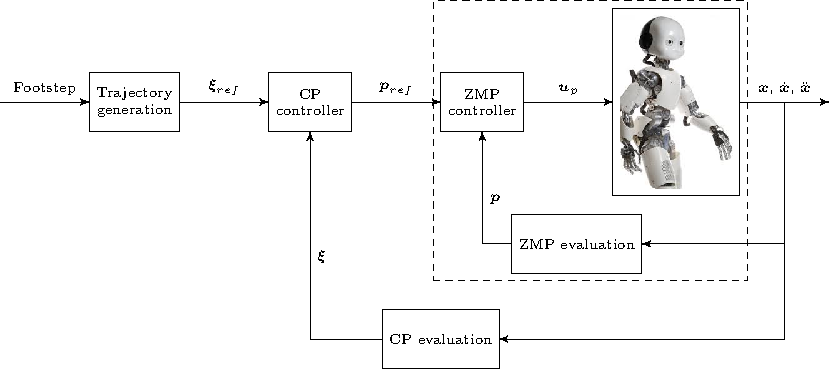
\includegraphics[scale=1.0]{control_architecture}
  \caption{Controller architecture. \label{fig:control_architecuture}}
\end{figure}
It is important to underline that in the controller synthesis the following assumption holds:
\begin{itemize}
\item[-] the position, velocity and acceleration of the CoM of the entire robot can be measured or,
  in general, derived;
\item[-] the jerk of the CoM $\dddot{\vec{x}}$ is the controlled input.
\end{itemize}

\subsection{Capture Point Controller}
Several version of capture point controller was proposed in these last years,
for example Englsberger proposed a linear feedback controller \cite{Englsberger2011}
while Krause a MPC approach \cite{Krause2012}.
Both of these architecture use the ZMP as the controlled variable and in order to respect the
constraints on the ZMP (see the principle \ref{principle:zmp}) in the linear controller approach
a projection inside the support polygon was proposed; while in the MPC approach the ZMP constraint
was incorporated in the MPC framework.
In the following dissertation the MPC approach is proposed.
\par
The aim of this approach is stabilizing only the unstable part of the CP dynamics
(\ref{eq:cp_dynamics}). The following dynamic equation is used as the prediction model
\begin{equation}
  \label{eq:cp_dynamics_vettorial}
  \dot{\vec{\xi}} = \omega(\vec{\xi} - \vec{p})
\end{equation}
where $\vec{\xi}$ is the vector that contains the $x$ and $y$ coordinates of the capture point,
while $\vec{p}$, the control input, contains the  $x$ and $y$ coordinates of the ZMP.
In the following a discrete time implementation with a piecewise constant control inputs.
The equation (\ref{eq:cp_dynamics_vettorial}) can be discretized
\[
\vec{\xi}_{k+1} = A \vec{\xi}_{k} + B \vec{p}_{k} =
\begin{bmatrix}
  e^{\omega T} & 0 \\
  0 & e^{\omega T} \\
\end{bmatrix}
\vec{\xi}_{k} +
\begin{bmatrix}
  1-e^{\omega T} \\
  1-e^{\omega T}
\end{bmatrix}
\vec{p}_{k} 
\]
where $T$ is the sampling time. In order to reduce the number of variable in the MPC problem the
``single shooting'' approach is used. The main idea is to keep only $\vec{\xi}_k$ and the vector
input $\vec{P}$ as variables and the states $\vec{\xi}_{k + 1}, \dots, \vec{\xi}_{k + N}$ are eliminated recursively.
Thus, the predicted capture point for the next $N$ states can be summarized as follows
\[
\vec{\Xi} = F_{\xi} \vec{\xi}_k + F_{p} \vec{P}
\]
where
\[
\vec{\Xi} =
\begin{bmatrix}
  \vec{\xi}_{k+1}\\
  \vdots\\
  \vec{\xi}_{k+N}
\end{bmatrix} \quad
\vec{P} =
\begin{bmatrix}
  \vec{p}_{k}\\
  \vdots\\
  \vec{p}_{k+N-1}
\end{bmatrix}
\]
and
\[
F_{\xi} =
\begin{bmatrix}
  A\\
  \vdots\\
  A^N
\end{bmatrix} \quad
F_p =
\begin{bmatrix}
  B & \hdots & 0\\
  \vdots &\ddots & \vdots\\
  A^{N-1} B & \hdots & B
\end{bmatrix}
\]
The control objective is the tracking the reference CP trajectory $\vec{\xi}_{ref}$ while the ZMP
position satisfies the well known constraint.
Thus the following objective function can be defined
\[
J_k = \frac{1}{2} \left\{  (\vec{\Xi}_{ref} - \vec{\Xi})\transpose Q (\vec{\Xi}_{ref} - \vec{\Xi}) +
(\Theta \vec{P} - \vec{e}_1 \vec{p}_{k-1}) \transpose R (\Theta \vec{P} - \vec{e}_1 \vec{p}_{k-1}) \right\}
\]
where $Q$ and $R$ are symmetric and positive definite matrices and $(\Theta \vec{P} - \vec{e}_1 \vec{p}_{k-1})$ is the rate of change of the controlled input. More specifically the matrix $\Theta$ is
defined as follow
\[
\Theta =
\begin{bmatrix}
  I & 0 & \hdots & 0 \\
  I & -I & \hdots & 0 \\
  \vdots & \vdots & \ddots & \vdots \\
  0 & 0 & \hdots & -I
\end{bmatrix}
\]
In order to embedded the ZMP constraint in the MPC framework the position the following inequality
must hold
\[
\vec{f}_{min} \le {}^f R_g(\alpha_k) ({}^g \vec{p}_k - {}^ g \vec{r}_k) \le \vec{f}_{max}
\]
where ${}^f R_g(\alpha_k)$ is the rotation matrix between the reference frame attached to the
reference foot and the global inertial frame (see Figure \ref{fig:control_architecuture});
$\vec{r}_k$ and $\alpha_k$ are respectively the footstep position and the orientation provided
by the footstep planning algorithm. Finally $\vec{f}_{min}$ and $\vec{f}_{max}$ are the minimum and
maximum values determined by rectangular envelope (draw in red in the figure
\ref{fig:control_architecuture}).
\begin{figure}[!ht]
  \centering
  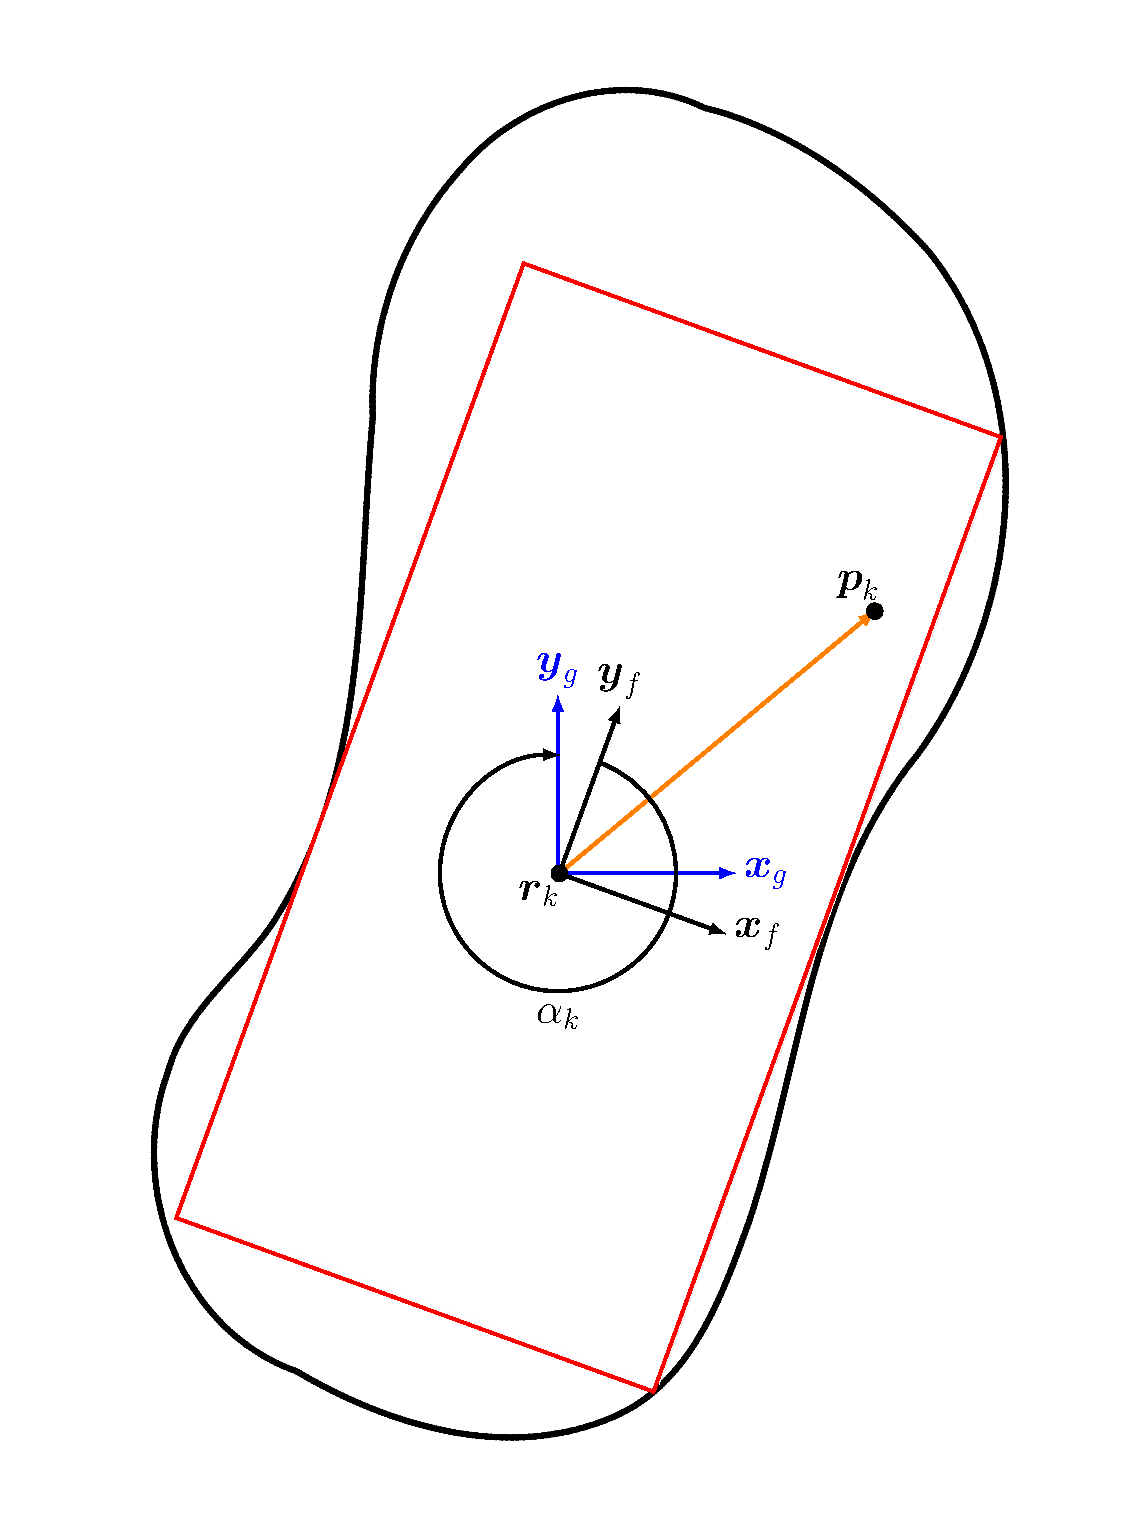
\includegraphics[scale=.4]{foot_support_polygon}
  \caption{Controller architecture. \label{fig:control_architecuture}}
\end{figure}
\par
In summary the following optimization problem has to be solved is
\[
\begin{split}
  \min_{\vec{P}, \vec{\xi}_k} &  \quad \left[  \frac{1}{2}\left\{ (\vec{\Xi}_{ref} - \vec{\Xi})\transpose Q (\vec{\Xi}_{ref} - \vec{\Xi}) + (\Theta \vec{P} - \vec{e}_1 \vec{p}_{k-1}) \transpose R (\Theta \vec{P} - \vec{e}_1 \vec{p}_{k-1}) \right\} \right]\\
  \text{s.t.} & \quad \quad \quad  F_{\xi} \vec{\xi}_k + F_{p} \vec{P}  - \vec{\Xi} = \vec{0}\\
  & \quad \quad \quad  \vec{f}_{min} \le {}^f R_g(\alpha_k) ({}^g \vec{p}_k - {}^ g \vec{r}_k) \le \vec{f}_{max}
\end{split}
\]
\subsection{Zero Momentum Point Controller}
In this section the inner zero momentum point controller is analyzed. This approach is based on the
Kajita work \cite{Kajita2003}.
Using the well known ZMP equations and the the fact that the two equation are decoupled
\[
\begin{split}
  p_y = y - \frac{z_c}{g} \ddot{y}\\
  p_x = x - \frac{z_c}{g} \ddot{y}
\end{split}
\]
the following dynamic system can be defined
\begin{equation}
  \label{eq:zmp_mpc}
  \begin{bmatrix}
    \dot{x} \\
    \ddot{x} \\
    \dddot{x}
  \end{bmatrix} =
  \begin{bmatrix}
    0 & 1 & 0 \\
    0 & 0 & 1 \\
    0 & 0 & 0
  \end{bmatrix}
  \begin{bmatrix}
    x \\
    \dot{x} \\
    \ddot{x}
  \end{bmatrix}
  +
  \begin{bmatrix}
    0 \\
    0 \\
    1 
  \end{bmatrix}
  u_x
\end{equation}
\begin{equation}
  \label{eq:zmp_mpc_y}
  p_x =
  \begin{bmatrix}
    1 & 0 & -\frac{z_c}{g}
  \end{bmatrix}
  \begin{bmatrix}
    x \\
    \dot{x} \\
    \ddot{x}
  \end{bmatrix}
\end{equation}
the same system can be obtained for the $y$-coordinate.
\par
An MPC controller can be synthesize using the equations \ref{eq:zmp_mpc} and \ref{eq:zmp_mpc_y}.
First of all the ZMP dynamic equation must be discretized with a fixed sampling time $T$.
\[
\begin{split}
  &\vec{x}_{k + 1} = A \vec{x}_k + B u_k\\
  &p_k = C \vec{x}_{k}
\end{split}
\]
where
\[
A = \begin{bmatrix}
  1 & T & \frac{T^2}{2}\\
  0 & 1 & T \\
  0 & 0 & 1
\end{bmatrix} \quad
B = \begin{bmatrix}
  \frac{T^3}{6}\\
  \frac{T^2}{2}\\
  T
\end{bmatrix}\quad
C =  \begin{bmatrix}
    1 & 0 & -\frac{z_c}{g}
  \end{bmatrix}
\]
The same approach shown in the previous section can be followed in order to formalize the optimal
problem.
Only $\vec{x}_k$ and the vector
input $\vec{U}$ as variables and the states $\vec{x}_{k + 1}, \dots, \vec{x}_{k + N}$ are eliminated recursively.
Thus, the predicted dynamic system for the next $N$ states can be summarized as follows
\[
\vec{X} = F_{x} \vec{x}_k + F_{u} \vec{U}
\]
where
\[
\vec{X} =
\begin{bmatrix}
  \vec{x}_{k+1}\\
  \vdots\\
  \vec{x}_{k+N}
\end{bmatrix} \quad
\vec{U} =
\begin{bmatrix}
  \vec{u}_{k}\\
  \vdots\\
  \vec{u}_{k+N-1}
\end{bmatrix}
\]
and
\[
F_{x} =
\begin{bmatrix}
  A\\
  \vdots\\
  A^N
\end{bmatrix} \quad
F_u =
\begin{bmatrix}
  B & \hdots & 0\\
  \vdots &\ddots & \vdots\\
  A^{N-1} B & \hdots & B
\end{bmatrix}
\]
While the output equation becomes
\[
\vec{P} = H_{x} \vec{x}_k + H_{u} \vec{U}
\]
where
\[
\vec{P} =
\begin{bmatrix}
  p_{k}\\
  \vdots\\
  p_{k+N}
\end{bmatrix}
\]
and
\[
H_{x} =
\begin{bmatrix}
  C \\
  CA \\
  \vdots\\
  C A^{N}
\end{bmatrix} \quad
H_u =
\begin{bmatrix}
  0 & 0 & \hdots & 0\\
  CB & 0 & \hdots &  0 \\
  CBA & CB & \hdots &  0 \\
  \vdots & \vdots & \ddots & \vdots \\ 
    CBA^{N-1} & CBA^{N-2} & \hdots &  C 
\end{bmatrix}
\]
The following objective function is chosen
\[
\frac{1}{2} \left\{ (\vec{P}_{ref} - \vec{P})\transpose Q_p (\vec{P}_{ref} - \vec{P}) +
\vec{\Delta U} \transpose R \vec{\Delta U} + 
\vec{\Delta X} \transpose Q_x \vec{\Delta x} \right\}
\]
where
\[
\vec{P} =
\begin{bmatrix}
  p_k \\
  p_{k + 1} \\
  \vdots \\
  p_{k + N -1}
\end{bmatrix} \quad
\vec{\Delta X} =
\begin{bmatrix}
  \vec{x}_k - \vec{x}_{k+1} \\
  \vec{x}_{k + 1} - \vec{x}_{k + 2} \\
  \vdots \\
  \vec{x}_{k + N - 1} - \vec{x}_{k + N}
\end{bmatrix} \quad
\vec{\Delta U} =
\begin{bmatrix}
  u_k - u_{k+1} \\
  u_{k + 1} - u_{k + 2} \\
  \vdots \\
  u_{k + N - 2} - u_{k + N - 1}
\end{bmatrix}
\]
while the matrix $Q_p$, $Q_x$ and $R$ are positive and non-negative definite matrix.
Last but not least the reference input $\vec{P}_{ref}$ is the output of the capture point controller
developed in the previus section.
\par
The MPC problem can be summarized as a Quadratic Programming Problem:
\[
\begin{split}
  \min_{\vec{U}, \vec{x}_k} &  \quad \left[\frac{1}{2} \left\{ (\vec{P}_{ref} - \vec{P})\transpose Q_p (\vec{P}_{ref} - \vec{P}) +
\vec{\Delta U} \transpose R \vec{\Delta U} + 
\vec{\Delta X} \transpose Q_x \vec{\Delta x} \right\} \right ]\\
  \text{s.t.} & \quad \quad \quad  F_{x} \vec{x}_k + F_{u} \vec{U} - \vec{X} = \vec{0}\\
  & \quad \quad \quad  H_{x} \vec{x}_k + H_{u} \vec{U} - \vec{P} = \vec{0}
\end{split}
\]


\newpage
\nocite{*}
\bibliography{bibliography}
\bibliographystyle{ieeetr}
\end{document}
